% !TeX root = ../main.tex

\section{Week 1: }

\newlecture[Set Theory Fundamentals][Sep 8, 2026]

``Probability = Set Theory + Measure''

\begin{enumerate}
    \item \textbf{Basic Set Operations}
    \\ Union, Intersect, Complement, \dots
    \\ $A\cup B,\ A\cap B,\ A^C, \dots$

    \item \deflabel{1.1.1}{Convergence of Real-Valued Sequences}
    \begin{quote}
        A sequence $(x_n)_{n=1}^\infty \subseteq \R$ converges to $x$ if
        \[\forall \varepsilon>0,\ \exists N \in \N \text{ s.t. } n>N \Rightarrow \left\lvert x_n-x\right\rvert < \varepsilon.\]
    \end{quote}
    $x_n \to x$ \aside{converge to $x$?}
    \\ \aside{Pick $\varepsilon$ (how close $x_n$ is to the target).}
    \\ For any $\varepsilon$ picked, can find $N$, such that $n>N$, $\left\lvert x_n-x\right\rvert < \varepsilon$.
    \\ e.g. $x_n = \dfrac{1}{n} \to 0$

    \item \deflabel{1.1.2}{Functional Convergence Pointwisely}
    \begin{quote}
        A sequence $(f_n)_{n=1}^\infty \subseteq \R^X$ converges pointwise to $f$ \aside{(target $f$)} if
        \[\forall \varepsilon>0,\ \forall x \in X,\ \exists N_x \in \N \text{ s.t. } n>N_x \Rightarrow \left\lvert f_n(x)-f(x)\right\rvert < \varepsilon.\]
    \end{quote}
    $f_1,\dots,f_n,\dots$ --- \aside{sequence of functions}
    \\ $f$ --- \aside{target function}
    \\ For any $\varepsilon$ and $x$, can find $N_x$ s.t. $n>N_x$, $\left\lvert f_n(x)-f(x)\right\rvert < \varepsilon$.
    \\ $f_1(2), f_2(2), \dots, f_n(2), \dots \to f(2)$ --- \aside{for every $x$, there is a corresponding $N_x$.}

    \item \deflabel{1.1.3}{Functional Convergence Uniformly}
    \begin{quote}
        A sequence $(f_n)_{n=1}^\infty \subseteq \R^X$ converges uniformly to $f$ if
        \[\forall \varepsilon>0,\ \hly{\exists N \in \N} \quad \forall x \in X,\ n>N \Rightarrow \left\lvert f_n(x)-f(x)\right\rvert < \varepsilon.\]
    \end{quote}
    \aside{That works for all $x \in X$ --- need a common threshold $N$ for uniform convergence.}
\end{enumerate}

\heading{Key difference:}
For pointwise convergence, you need to have $x$ specified first, then there is a threshold $N_x$ corresponding to each $x$.
\\ For uniform convergence, you need a common threshold $N$ that works for all $x \in X$.

\begin{example}
    \[f_n(x) = \frac{x}{n+x}, \quad x\geq 0\]
    Then for any fixed value $x$, as $n\to\infty$, $f_n(x)\to 0$:
    \\ $x=1$: $f_n(1) = \dfrac{1}{n+1} \to 0$ as $n\to\infty$.
    \\ $x=2$: $f_n(2) = \dfrac{2}{n+2} \to 0$ as $n\to\infty$.
    \[\therefore f_n(x) \xrightarrow{\text{pointwise}} 0\]

    However, $f_n$ does not converge uniformly to $0$: no $N$ works for all $x$.
    \\ No matter how you specify $N$, there is always a larger value of $x$ for which the bound fails.
    \[\Rightarrow f_n(x) \not\xrightarrow{\text{uniformly}} 0\]
\end{example}

\subsection{Limiting Processes}

\deflabel{1.2.1}{The Supremum of a Set}
\begin{quote}
    Let $A \subseteq \R$ be a subset. $u = \sup A$ iff
    \[\forall \varepsilon>0,\ \exists x \in A \quad u-x<\varepsilon \quad \text{and} \quad \forall x \in A,\ x \leq u.\]
\end{quote}

\deflabel{1.2.2}{The Infimum of a Set}
\begin{quote}
    Let $A \subseteq \R$ be a subset. $v = \inf A$ iff
    \[\forall \varepsilon>0,\ \exists x \in A \quad x-v<\varepsilon \quad \text{and} \quad \forall x \in A,\ x \geq v.\]
\end{quote}

\begin{center}
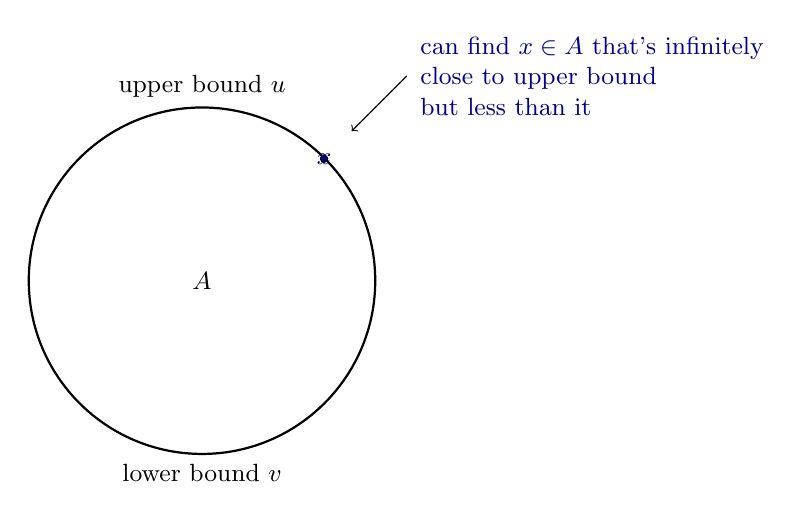
\begin{tikzpicture}[scale=1, every node/.style={font=\small}]
    \draw[thick] (0,0) circle (2.2cm);
    \node at (0,0) {$A$};
    \node[blue!55!black] at (1.55,1.55) {$x$};
    \draw[fill=blue!55!black] (1.55,1.55) circle (1.3pt);
    \node[above] at (0,2.2) {upper bound $u$};
    \node[below] at (0,-2.2) {lower bound $v$};
    \draw[->] (2.6,2.6) -- (1.9,1.9);
    \node[align=left, blue!55!black, anchor=west] at (2.65,2.6) {\aside{\shortstack[l]{can find $x \in A$ that's infinitely\\ close to upper bound\\ but less than it}}};
\end{tikzpicture}
\end{center}

\begin{example}
    \[A = (0,1)\]
    \[\sup A = 1 \qquad \inf A = 0\]
\end{example}

\heading{Distinction of sup/inf vs.\ max/min:}
$\max(A)$ and $\min(A)$ must be elements of the set $A$.
\\ $\sup(A)$ and $\inf(A)$ may not be elements of $A$.

\begin{example}
    \[A = (0,1)\]
    $\max(A)$ and $\min(A)$ do not exist. $\sup(A)$ and $\inf(A)$ do exist.
    \[B = (0,1]\]
    $\min(B)$ does not exist, $\max(B) = 1$. $\sup(B) = 1$, $\inf(B) = 0$.
\end{example}

\deflabel{1.2.3}{Limsup and Liminf}
\begin{quote}
    Let $(x_n) \subseteq \R$ be a sequence.
    \[\limsup_{n\to\infty} x_n = \lim_{n\to\infty}\ \sup_{m\geq n} x_m = \inf_{n\geq 0}\ \sup_{m\geq n} x_m\]
    \[\liminf_{n\to\infty} x_n = \lim_{n\to\infty}\ \inf_{m\geq n} x_m = \sup_{n\geq 0}\ \inf_{m\geq n} x_m\]
\end{quote}

\begin{center}
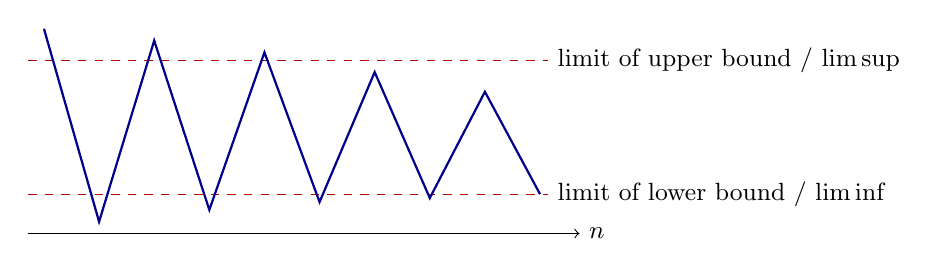
\begin{tikzpicture}[scale=1, every node/.style={font=\small}]
    \draw[->] (0,0) -- (7,0) node[right]{$n$};
    \draw[dashed, red!70!black] (0,2.2) -- (6.6,2.2) node[right, black]{\aside{limit of upper bound / $\limsup$}};
    \draw[dashed, red!70!black] (0,0.5) -- (6.6,0.5) node[right, black]{\aside{limit of lower bound / $\liminf$}};
    \draw[thick, blue!55!black]
        (0.2,2.6) -- (0.9,0.15) -- (1.6,2.45) -- (2.3,0.3) -- (3,2.3)
        -- (3.7,0.4) -- (4.4,2.05) -- (5.1,0.45) -- (5.8,1.8) -- (6.5,0.5);
\end{tikzpicture}
\end{center}

\begin{example}
    \[x_n = (-1)^n = -1,1,-1,1,\dots\]
    No limit, diverges: $\displaystyle\lim_{n\to\infty} x_n$ DNE.
    \\ But $\displaystyle\sup_{m\geq n} x_m = 1$ and $\displaystyle\inf_{m\geq n} x_m = -1$
    \[\Rightarrow \limsup_{n\to\infty} x_n = 1, \qquad \liminf_{n\to\infty} x_n = -1\]
\end{example}

\aside{The limsup and liminf are used to describe the long-run behaviour of a sequence, even if the sequence does not converge.}
\\ For a sequence $x_n$, if $\displaystyle\limsup_{n\to\infty} x_n = \liminf_{n\to\infty} x_n = x$, then $\displaystyle\lim_{n\to\infty} x_n = x$.

\subsection{Function Limits}

\deflabel{1.3}{Left and Right Limit of a Function}
\begin{quote}
    For any function $f: \R \to \R$,
    \[f(x-) = \lim_{y\uparrow x} f(y) = L \quad \aside{(to the left of $x$, a small neighbourhood)}\]
    \[\Leftrightarrow \forall \varepsilon>0,\ \exists \delta>0 \text{ s.t. } \forall y \in (x-\delta,x),\ \left\lvert f(y)-L\right\rvert < \varepsilon.\]
    \[f(x+) = \lim_{y\downarrow x} f(y) = U\]
    \[\Leftrightarrow \forall \varepsilon>0,\ \exists \delta>0 \text{ s.t. } \forall y \in (x,x+\delta),\ \left\lvert f(y)-U\right\rvert < \varepsilon.\]
    If $f(x-) = f(x+) = C$, then $\textcolor{blue!55!black}{\displaystyle\lim_{y\to x} f(y) = C}$.
\end{quote}

\begin{example}
    \[f(x) = \begin{cases} 0 & x<0 \\ 1 & x\geq 0 \end{cases}\]
    $f(0-) = 0$, $f(0+) = 1$
    \[\Rightarrow \lim_{x\to 0} f(x) \text{ DNE}\]
\end{example}


\newlecture[Probability Measure][Sep 10, 2026]

\deflabel{2.1}{Sample Space}
\begin{quote}
    A sample space $\Omega$ is any non-empty set.
\end{quote}

\begin{example}
    The sample space contains ''all the states of the following''
    \\Coin Flipping: $\Omega: \{H, T\}$
    \\Weather: $\{\text{hot, cold, mild}\} \times \{\text{wet, dry}\}$
\end{example}

\deflabel{2.2}{Probability Measure (STA347 ver.)}
\begin{quote}
    For a sample space $\Omega$, we say $P$ is a probability measure if the following holds:
    \begin{enumerate}[label=\roman*)]
        \item $\forall E \subseteq \Omega, 0 \leq P(E) \leq 1$, that is $P:\mathcal{P}(\Omega) \to [0,1]$
        \item $P(\Omega) = 1$
        \item $\forall E_1, E_2, \dots \subseteq \Omega$ such that $E_i \cap E_j = \varnothing \ \forall\ i \neq j$
        \[P\left(\bigcup_{i=1}^{\infty} E_i\right) = \sum_{i=1}^{\infty}P(E_i)\]
    \end{enumerate}
\end{quote}

\aside{$\mathcal{P}(\Omega)$ is the power set of $\Omega$.}

\textbf{Remark:} It may be impossible for such a $P$ to exist. To define exactly which subsets we want $P$ to satisfy these axioms, that would require more advanced mathematical theories. For this class, we just assume such a $P$ is defined for all subsets of $\Omega$.

\begin{example}
    Probabilities of coin flipping
    \[\Omega = \{H, T\}\]
    \[\mathcal{P}(\Omega) = \{\phi, \{H\}, \{T\}, \{H, T\}\}\]
    \[P: \mathcal{P}(\Omega) \mapsto [0, 1]\]
    \begin{align*}
        p: \phi &\mapsto 0 \\
        \{H\} &\mapsto \frac{1}{2} \\
        \{T\} &\mapsto \frac{1}{2} \\
        \{H, T\} &\mapsto 1
    \end{align*}
\end{example}

\begin{example}
    The uniform/Lebesgue measure.
    Let $\Omega =[L,U]$ for some $L < U \in \R$. Define
    \[P([a,b]) = \frac{b-a}{U-L} \quad \text{when } L \leq a \leq b \leq U\]
    We assume such a measure exists (and is well defined) for this class.
\end{example}

Proposition 2.3:
The following properties are satisfied by any probability measure $P$
\begin{enumerate}
    \item $\forall E \subseteq \Omega, P(E^C) = 1 - P(E)$
    \item $P(\phi) = 0$
    \item $\forall E, F \subseteq \Omega$, such that $E \subseteq F, P(E) \leq P(F)$ \aside{(``big event, big probability'')}
    \item $\forall E, F \subseteq \Omega, P(E\bigcup F) = P(E)+P(F) - P(E\bigcap F)$
    \item $\forall E, F \subseteq \Omega, P(E\bigcap F) = P(E)+P(F)-P(E\bigcup F)$
    \item $\forall E, F \subset \Omega, P(F \setminus E) = P(F) - P(E\bigcap F)$
\end{enumerate}

Proof via Def 2.2 (probability axioms).

Lemma 2.4
\begin{quote}
    For a sequence $E_1, \dots, E_n \subseteq \Omega$
    \[P(\bigcup_{i=1}^n E_i) \leq \sum_{i=1}^{n}P(E_i)\]
    Proof: We define $F_i = E_i \setminus \bigcup_{j=1}^{i-1}E_j, F_1 = E_1$
    \[\bigcup_{i=1}^{n} E_i = \bigcup_{i=1}^{n}F_i \text{ and } F_i \bigcap F_j = \phi \text{ if } i \neq j\]
    from the probability axiom.
    \begin{align*}
        \text{Since } \bigcup_{i=1}^{n} E_i &= \bigcup_{i=1}^{n}F_i\\
        P(\bigcup_{i=1}^{n} E_i) &= P(\bigcup_{i=1}^{n}F_i)\\
        &= \sum_{i=1}^{n}P(F_i)
    \end{align*}
    \[\text{We also know } F_i \subseteq E_i \text{ as } F_i = E_i \setminus \bigcup_{j=1}^{i-1}E_j\]
    \[P(F_i) \leq P(E_i)\]
    \[P(\bigcup_{i=1}^{n}E_i) = \sum_{i=1}^{n}P(F_i) \leq \sum_{i=1}^{n}P(E_i)\]
\end{quote}

Lemma 2.5
\begin{quote}
    Let $P$ be the Lebesgue measure on $[0,1]$. Then $P(E) = 0$ for any \underline{countable} set $E$.
\end{quote}